\documentclass{article}
\usepackage{graphicx}
\usepackage{algorithm}
\usepackage{algpseudocode}
\usepackage{amsmath}
\usepackage{ulem}
\usepackage{booktabs}
\usepackage{caption}
\usepackage{tikz}
\usetikzlibrary{shapes.gates.logic.US, calc}
\usepackage[margin=1in]{geometry}

\title{Technical Communication - Assignment 6}
\author{UTKARSH KUMAR 23114101}
\date{March 2026}

\begin{document}

\maketitle

\begin{enumerate}
    \item 
\begin{enumerate}
    \item 
\textbf{Algorithm in \LaTeX with Filled Blanks}
\begin{algorithm}[H]
\caption{Dijkstra's Algorithm}

\begin{algorithmic}[]

\State For each vertex $v \in V$:
    \State \qquad \texttt{dist}$[v] \gets \infty$,\qquad \texttt{visited}$[v] \gets \text{False}$
\State Then set:
    \State \qquad \texttt{dist}$[s] \gets 0$
    
\State Repeat for $|V|$ iterations:
    \State \qquad \textbullet\ choose the unvisited vertex $u$ with minimum \texttt{dist}[$u$]
    \State \qquad \textbullet\ if \texttt{dist}$[u] = \infty$, stop
    \State \qquad \textbullet\ set \texttt{visited}$[u] \gets \text{True}$
    \State \qquad \textbullet\ for each neighbor $v$ of $u$ in alphabetical order:
    
    \State \qquad \qquad -- if \texttt{visited}$[v] = \text{False}$ and \texttt{dist}$[u] + w(u, v) < \texttt{dist}[v]$
    \State \qquad \qquad -- then set \texttt{dist}$[v] \gets \texttt{dist}[u] + w(u, v)$
\State Return \texttt{dist}
\end{algorithmic}
\end{algorithm}

\item \textbf{Execution Table in \LaTeX with Filled Entries}
\begin{table}[h]
    \centering
    \begin{tabular}{c|c|c}
        \toprule
        Step & Finalized Node & Distance Vector $(A, B, C, D, E, F)$ \\
        \midrule
        0 & -- & $(0, \infty, \infty, \infty, \infty, \infty)$ \\
        1 & A & $(0, 4, 2, \infty, \infty, \infty)$ \\
        2 & C & $(0, 3, 2, 10, 12, \infty)$ \\
        3 & B & $(0, 3, 2, 8, 12, \infty)$ \\
        4 & D & $(0, 3, 2, 8, 10, 14)$ \\
        5 & E & $(0, 3, 2, 8, 10, 13)$ \\
        6 & F & $(0, 3, 2, 8, 10, 13)$ \\
        \bottomrule
    \end{tabular}
    \caption{Distance Table}
\end{table}

\item \textbf{Final Result in \LaTeX}

Shortest distance from A to F = 13 \\
Shortest path from A to F = A $\rightarrow$ C $\rightarrow$ B $\rightarrow$ D $\rightarrow$ E $\rightarrow$ F

\item \textbf{Precision Statement in \LaTeX}

In Dijkstra's Algorithm, the relaxation step checks whether \uline{a new discovered path to a vertex is shorter than the previously known shortest path}. If the condition \uline{$\texttt{dist}[u] + w(u,v) < \texttt{dist}[v]$} holds, the algorithm updates \uline{$\texttt{dist}[v]$ to $\texttt{dist}[u] + w(u,v)$}.
\end{enumerate}

\newpage

\item 
In the following, we show how to use the \texttt{minipage} environment to combine text and logic circuit diagrams as shown in fig.1.

\vspace{0.5cm}

\begin{minipage}[t]{0.52\textwidth}
    \vspace{30pt}
    \centering
    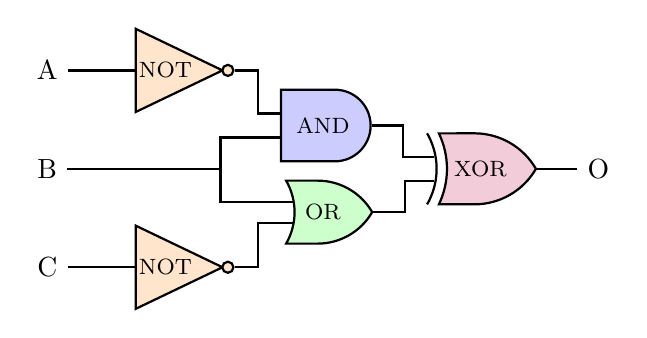
\begin{tikzpicture}[
        thick,
        gate/.style={draw, thick, minimum width=1cm, minimum height=0.8cm},
        not gate/.style={not gate US, gate, fill=orange!20},
        and gate/.style={and gate US, gate, fill=blue!20},
        or gate/.style={or gate US, gate, fill=green!20},
        xor gate/.style={xor gate US, gate, fill=purple!20}
    ]
    
        \node (A) at (0, 2.5) {A};
        \node (B) at (0, 1.25) {B};
        \node (C) at (0, 0) {C};

        \node[not gate] (nA) at (1.5, 2.5) {\footnotesize NOT};
        \node[not gate] (nC) at (1.5, 0)   {\footnotesize NOT};
        \node[and gate] (a1) at (3.5, 1.8) {\footnotesize AND};
        \node[or gate]  (o1)  at (3.5, 0.7) {\footnotesize OR};
        \node[xor gate] (x1) at (5.5, 1.25) {\footnotesize XOR};
        \node (O)  at (7, 1.25) {O};
        
        \draw (A) -- (nA.input);
        \draw (C) -- (nC.input);
        \draw (nA.output) -- ++(0.3,0) |- (a1.input 1);
        \draw (nC.output) -- ++(0.3,0) |- (o1.input 2);
        \draw (B) -- (2.2, 1.25) coordinate (Bs);
        \draw (Bs) |- (a1.input 2);
        \draw (Bs) |- (o1.input 1);
        \draw (a1.output) -- ++(0.4,0) |- (x1.input 1);
        \draw (o1.output) -- ++(0.4,0) |- (x1.input 2);
        \draw (x1.output) -- (O);
    \end{tikzpicture}
    \captionof{figure}{Combinational Logic Circuit}
\end{minipage}
\hfill
\begin{minipage}[t]{0.45\textwidth}
    \vspace{0pt}
    \textbf{Digital Logic Design}\\
    The logic circuit shown in the image is a combinational system that processes three binary inputs (A, B, and C) through three stages of logic to determine the final output O. In the first stage, inputs A and C are passed through NOT gates to create their inverted complements, $\neg A$ and $\neg C$. Next, an AND gate combines $\neg A$ with input B, while an OR gate combines input B with $\neg C$. Finally, these two intermediate results are fed into an XOR (Exclusive OR) gate, which produces a "True" output only if the signals from the AND and OR stages are different. The overall behavior can be summarized by the Boolean expression $O = (\neg A \land B) \oplus (B \lor \neg C)$.
\end{minipage}

\end{enumerate}
\end{document}

